% !TEX root = ../main.tex
\chapter{The Geometry of Linear Equations}
\label{ch:1}

The fundamental problem of linear algebra is to solve a system of $n$ linear equations in $n$ unknowns. That problem is so familiar from school --- two lines, find where they cross --- that it is easy to think there is nothing left to understand. There is. The whole course turns on \emph{seeing} a linear system the right way, and the right way is not the one most of us were taught.

Take the smallest interesting example, two equations in two unknowns:
\begin{equation}\label{eq:ch1-2by2}
\ba
2x - y &= 0, \\
-x + 2y &= 3.
\ea
\end{equation}
There are three ways to look at this system, and we will use all three throughout the book. The \emph{row picture} plots one line per equation and asks where they meet --- this is the picture you already know. The \emph{column picture} reads the same numbers down the columns instead of across the rows, and asks a different question: how do we combine two fixed vectors to produce a third? This second picture is the one to fall in love with. Almost everything later --- column space, rank, independence, the four fundamental subspaces --- is the column picture growing up. The \emph{matrix picture} then packages everything as $Ax=b$, and the real content of the chapter is learning to read those three symbols in two different ways at once.

\section{The Row Picture}

In the row picture we take the equations one at a time. Each equation in two unknowns describes a line in the $xy$-plane, namely all points $(x,y)$ that satisfy it. A solution of the \emph{system} must satisfy \emph{every} equation, so it is a point lying on \emph{all} the lines at once --- a point of intersection.

For the system~\eqref{eq:ch1-2by2}, the first equation $2x-y=0$ is the line $y=2x$ through the origin; the second, $-x+2y=3$, is the line $y=\tfrac12 x+\tfrac32$. They cross at a single point, and reading it off (or solving the two equations by hand) gives
\[
x=1,\qquad y=2.
\]
We check by substituting back: $2(1)-2=0$ and $-1+2(2)=3$. Both hold, so $(1,2)$ is the solution.

\begin{center}
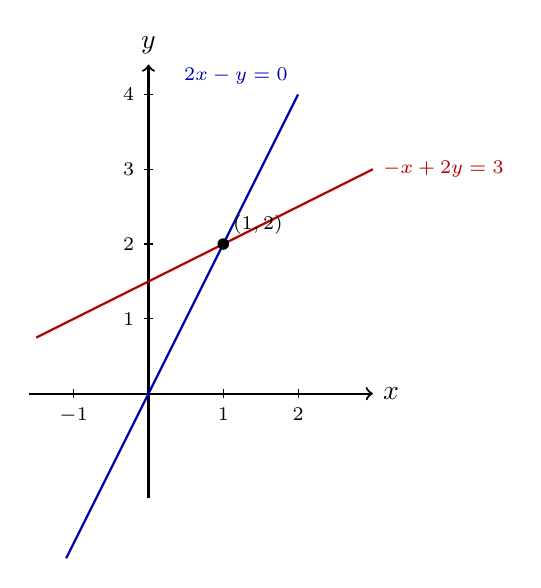
\begin{tikzpicture}[scale=0.95]
  % axes
  \draw[->,thick] (-1.6,0) -- (3.0,0) node[right]{$x$};
  \draw[->,thick] (0,-1.4) -- (0,4.4) node[above]{$y$};
  \foreach \x in {-1,1,2} \draw (\x,0.06)--(\x,-0.06) node[below,font=\scriptsize]{$\x$};
  \foreach \y in {1,2,3,4} \draw (0.06,\y)--(-0.06,\y) node[left,font=\scriptsize]{$\y$};
  % line 1: y = 2x  (2x - y = 0)
  \draw[thick,blue!70!black,domain=-1.1:2.0] plot (\x,{2*\x})
        node[above left,font=\scriptsize,blue!70!black] {$2x-y=0$};
  % line 2: y = x/2 + 3/2  (-x + 2y = 3)
  \draw[thick,red!70!black,domain=-1.5:3.0] plot (\x,{0.5*\x+1.5})
        node[right,font=\scriptsize,red!70!black] {$-x+2y=3$};
  % intersection
  \fill (1,2) circle (2.2pt) node[above right,font=\scriptsize] {$(1,2)$};
\end{tikzpicture}
\end{center}

Nothing here is new. The point of the row picture is that it stops being helpful exactly when we need it most. With three unknowns, each equation becomes a \emph{plane} in $\RR^3$, and the solution is where three planes meet --- typically in a single point, but two planes meet in a line, and the third plane may or may not pass through it. With ten unknowns we are intersecting ten hyperplanes in $\RR^{10}$, and no one can see that. We need a picture that scales. That picture comes from reading the columns.

\section{The Column Picture}

Look at the same system~\eqref{eq:ch1-2by2} again, but now collect the coefficients down the \emph{columns} rather than across the rows. The two numbers multiplying $x$ are $2$ and $-1$; the two multiplying $y$ are $-1$ and $2$; the right-hand sides are $0$ and $3$. So the system says exactly
\begin{equation}\label{eq:ch1-colpic}
x\begin{bmatrix} 2\\ -1\end{bmatrix}
+ y\begin{bmatrix} -1\\ 2\end{bmatrix}
= \begin{bmatrix} 0\\ 3\end{bmatrix}.
\end{equation}
This is the \emph{same two equations} --- read off the top entries and you recover $2x-y=0$; read off the bottom entries and you recover $-x+2y=3$. But the question has changed completely. We are no longer asking ``where do two lines cross?'' We are asking: \emph{how much of each column vector do we need so that they add up to the right-hand side?}

\defn{Linear Combination}{{Given vectors $v_1,\dots,v_n$ in $\RR^m$ and scalars $x_1,\dots,x_n$, the vector
\[
x_1 v_1 + x_2 v_2 + \cdots + x_n v_n
\]
is called a \emph{linear combination} of $v_1,\dots,v_n$. To take combinations of vectors --- scale them and add them --- is the one fundamental operation of the whole subject.}}


So solving the system means finding the scalars $x$ and $y$ that make the linear combination $x\,(2,-1)+y\,(-1,2)$ land on $(0,3)$. We already know the answer must be $x=1,\,y=2$, and we can watch it work:
\[
1\begin{bmatrix} 2\\ -1\end{bmatrix}
+ 2\begin{bmatrix} -1\\ 2\end{bmatrix}
= \begin{bmatrix} 2\\ -1\end{bmatrix}
+ \begin{bmatrix} -2\\ 4\end{bmatrix}
= \begin{bmatrix} 0\\ 3\end{bmatrix}.\quad\checkmark
\]
Geometrically, one copy of the first column followed by two copies of the second forms a little path from the origin to the target $b=(0,3)$.

\begin{center}
\begin{tikzpicture}[scale=0.82,>=Stealth]
  \draw[->,gray] (-3.4,0)--(1.6,0) node[right,font=\scriptsize]{};
  \draw[->,gray] (0,-1.6)--(0,4.4) node[above,font=\scriptsize]{};
  % first column (2,-1) from origin
  \draw[->,very thick,blue!70!black] (0,0)--(2,-1)
       node[midway,below right,font=\scriptsize] {$\begin{bmatrix}2\\-1\end{bmatrix}$};
  % from (2,-1) add 2*(-1,2) = (-2,4) -> ends at (0,3)
  \draw[->,very thick,red!70!black] (2,-1)--(0,3);
  \node[red!70!black,font=\scriptsize] at (1.55,1.4) {$2\begin{bmatrix}-1\\2\end{bmatrix}$};
  % resultant b
  \draw[->,very thick,black,dashed] (0,0)--(0,3);
  \fill (0,3) circle (2pt) node[left,font=\scriptsize] {$b=\begin{bmatrix}0\\3\end{bmatrix}$};
\end{tikzpicture}
\end{center}

Now ask the deeper question. We solved this for one particular $b=(0,3)$. What if the right-hand side were some \emph{other} vector? Could we still hit it with a combination of the two columns $(2,-1)$ and $(-1,2)$? In two dimensions the answer is yes for \emph{every} $b$: these two columns point in genuinely different directions, and their combinations $x(2,-1)+y(-1,2)$ sweep out the entire plane. Every vector in $\RR^2$ is reachable, so $Ax=b$ is solvable for every $b$. That ``filling the whole space'' is the property we will spend the next chapters naming and measuring.

\rmkb[Why the column picture wins]{
The row picture and the column picture contain identical information --- the same coefficients, just read in two directions. But the column picture answers the questions that organize the rest of the course. ``Which right-hand sides $b$ can I reach?'' becomes ``which vectors are combinations of the columns?'' --- that set will be the \emph{column space} (Chapter~\ref{ch:4}). ``Is the solution unique?'' becomes ``can a nonzero combination of the columns give zero?'' --- that is \emph{linear independence}. Keep one eye on the columns from now on.}


\section{The Matrix Picture: \texorpdfstring{$Ax=b$}{Ax=b}}

The two columns and the right-hand side are begging to be packaged. Put the columns of coefficients side by side into a \emph{matrix} $A$, stack the unknowns into a vector $x$, and the right-hand sides into a vector $b$:
\[
A=\begin{bmatrix} 2 & -1\\ -1 & 2\end{bmatrix},\qquad
x=\begin{bmatrix} x\\ y\end{bmatrix},\qquad
b=\begin{bmatrix} 0\\ 3\end{bmatrix}.
\]
The matrix $A$ is the \emph{coefficient matrix}; its columns are exactly the vectors from~\eqref{eq:ch1-colpic}. The entire system collapses to three symbols:
\[
\boxed{\,Ax=b.\,}
\]
For a general $m\times n$ system --- $m$ equations, $n$ unknowns --- we write $A\in\RR^{m\times n}$, $x\in\RR^n$, $b\in\RR^m$. The matrix $A$ has one row per equation and one column per unknown.

Everything now depends on what the product $Ax$ \emph{means}. There are two ways to compute it, and the difference between them is the difference between the two pictures.

\subsection{Two ways to read \texorpdfstring{$Ax$}{Ax}}

Consider a concrete product, with the unknowns set to $x=(1,2)$:
\[
\begin{bmatrix} 2 & 5\\ 1 & 3\end{bmatrix}
\begin{bmatrix} 1\\ 2\end{bmatrix}=\ ?
\]

\textbf{Reading 1: rows (the dot-product view).} Take each row of $A$ and dot it with $x$. The first row $(2,5)$ against $(1,2)$ gives $2\cdot1+5\cdot2=12$; the second row $(1,3)$ against $(1,2)$ gives $1\cdot1+3\cdot2=7$:
\[
\begin{bmatrix} 2 & 5\\ 1 & 3\end{bmatrix}
\begin{bmatrix} 1\\ 2\end{bmatrix}
=\begin{bmatrix} 2\cdot1+5\cdot2\\ 1\cdot1+3\cdot2\end{bmatrix}
=\begin{bmatrix} 12\\ 7\end{bmatrix}.
\]
This is the mechanical rule everyone learns, and it is the row picture in disguise: each entry of $Ax$ is one equation's left-hand side.

\textbf{Reading 2: columns (the combination view).} Treat the entries of $x$ as the amounts of each column. One copy of the first column plus two copies of the second:
\[
\begin{bmatrix} 2 & 5\\ 1 & 3\end{bmatrix}
\begin{bmatrix} 1\\ 2\end{bmatrix}
=1\begin{bmatrix} 2\\ 1\end{bmatrix}+2\begin{bmatrix} 5\\ 3\end{bmatrix}
=\begin{bmatrix} 2\\ 1\end{bmatrix}+\begin{bmatrix} 10\\ 6\end{bmatrix}
=\begin{bmatrix} 12\\ 7\end{bmatrix}.
\]
Same answer, of course. But this reading says something the first one hides: $Ax$ is a \emph{linear combination of the columns of $A$}, with the entries of $x$ as the coefficients. This is the single most important sentence in the chapter.

\state{The meaning of $Ax$}{
For $A\in\RR^{m\times n}$ with columns $a_1,\dots,a_n$ and $x=(x_1,\dots,x_n)\T$,
\[
Ax=x_1 a_1 + x_2 a_2 + \cdots + x_n a_n .
\]
The product $Ax$ is the linear combination of the columns of $A$ weighted by the entries of $x$. Solving $Ax=b$ asks: \emph{which combination of the columns produces $b$?}}


\subsection{When does \texorpdfstring{$Ax=b$}{Ax=b} have a solution?}

Reading $Ax$ as a combination of columns answers the existence question immediately. As $x$ ranges over all of $\RR^n$, the products $Ax$ range over \emph{all} linear combinations of the columns of $A$. So $Ax=b$ has a solution precisely when $b$ is one of those combinations.

\defn{Column Space}{{The \emph{column space} of $A\in\RR^{m\times n}$, written $\Col{A}$, is the set of all linear combinations of the columns of $A$:
\[
\Col{A}=\set{\,Ax : x\in\RR^n\,}\subseteq\RR^m .
\]
It is the set of all right-hand sides $b$ that the columns can reach.}}


\prop{Solvability of $Ax=b$}{{The system $Ax=b$ has a solution if and only if $b$ lies in the column space $\Col{A}$.}}

\pf{
If $Ax=b$ for some $x$, then $b=Ax$ is by definition a linear combination of the columns, so $b\in\Col{A}$. Conversely, if $b\in\Col{A}$ then $b=x_1a_1+\cdots+x_na_n$ for some scalars $x_i$; collecting those scalars into $x=(x_1,\dots,x_n)\T$ gives $Ax=b$.}


For the $2\times2$ matrix $A=\left[\begin{smallmatrix}2&-1\\-1&2\end{smallmatrix}\right]$, the two columns point in different directions and their combinations fill all of $\RR^2$; the column space is the whole plane, so $Ax=b$ is solvable for every $b$ --- and, because the columns are independent, the solution is unique. When a square matrix has this property we call it \emph{invertible}, and we may solve in one stroke by writing $x=A^{-1}b$ (we build $A^{-1}$ in Chapter~\ref{ch:2}). The clean case is the one where the columns fill the space; the rest of this chapter is about what goes wrong when they do not.

\section{Three Equations, Three Unknowns}

The two pictures grow up gracefully. In $\RR^3$ each equation is a plane (the row picture), and $Ax$ is a combination of three column vectors in space (the column picture). A good way to feel the difference is Strang's \emph{difference matrix}, where the columns have meaning.

\ex[A difference matrix]{
Take the three columns
\[
u=\begin{bmatrix} 1\\ -1\\ 0\end{bmatrix},\quad
v=\begin{bmatrix} 0\\ 1\\ -1\end{bmatrix},\quad
w=\begin{bmatrix} 0\\ 0\\ 1\end{bmatrix},
\qquad
A=\begin{bmatrix} 1 & 0 & 0\\ -1 & 1 & 0\\ 0 & -1 & 1\end{bmatrix},
\]
so $A$ has $u,v,w$ as its columns. Multiplying gives
\[
Ax=\begin{bmatrix} 1 & 0 & 0\\ -1 & 1 & 0\\ 0 & -1 & 1\end{bmatrix}
\begin{bmatrix} x_1\\ x_2\\ x_3\end{bmatrix}
=\begin{bmatrix} x_1\\ x_2-x_1\\ x_3-x_2\end{bmatrix}
= x_1 u + x_2 v + x_3 w .
\]
The output records the \emph{differences} of consecutive components of $x$ --- that is why $A$ is called a difference matrix. Now solve $Ax=b$. The equations
\[
\ba
x_1 &= b_1,\\
x_2-x_1 &= b_2,\\
x_3-x_2 &= b_3
\ea
\]
unwind from the top: $x_1=b_1$, then $x_2=b_1+b_2$, then $x_3=b_1+b_2+b_3$. The solution \emph{sums} the right-hand side:
\[
x=\begin{bmatrix} b_1\\ b_1+b_2\\ b_1+b_2+b_3\end{bmatrix}
=\begin{bmatrix} 1 & 0 & 0\\ 1 & 1 & 0\\ 1 & 1 & 1\end{bmatrix} b
= A^{-1}b .
\]
A solution exists for \emph{every} $b\in\RR^3$, and it is unique --- difference and sum undo each other, so $A^{-1}$ is the \emph{sum matrix}. The three columns $u,v,w$ are independent and their combinations fill all of $\RR^3$; the column space is the whole space. When that happens for $n$ vectors in $\RR^n$, we say they form a \emph{basis} for $\RR^n$, and the matrix holding them is invertible.}


\section{Singular Matrices: When the Columns Are Dependent}

So far the columns have always filled the space, and life is easy. The interesting --- and, for real problems, the usual --- case is when they do not. Change just one column of the difference matrix and the whole story changes.

\ex[A circular difference matrix]{
Replace the last column so that the differences ``wrap around'':
\[
C=\begin{bmatrix} 1 & 0 & -1\\ -1 & 1 & 0\\ 0 & -1 & 1\end{bmatrix},
\qquad
Cx=\begin{bmatrix} x_1-x_3\\ x_2-x_1\\ x_3-x_2\end{bmatrix}.
\]
Two things are different now. First, $Cx=0$ has nonzero solutions: if $x_1=x_2=x_3$ then every difference vanishes, so $Cx=0$ for the whole line of vectors $x=(c,c,c)$. The combination
\[
1\cdot\!\begin{bmatrix} 1\\ -1\\ 0\end{bmatrix}+1\cdot\!\begin{bmatrix} 0\\ 1\\ -1\end{bmatrix}+1\cdot\!\begin{bmatrix} -1\\ 0\\ 1\end{bmatrix}=\begin{bmatrix} 0\\ 0\\ 0\end{bmatrix}
\]
shows the three columns are \emph{linearly dependent} --- a nontrivial combination of them gives zero. Because we cannot reverse this collapse, no inverse $C^{-1}$ exists.

Second, $Cx=b$ is not solvable for every $b$. Add the three equations
\[
\ba
x_1-x_3 &= b_1,\\
x_2-x_1 &= b_2,\\
x_3-x_2 &= b_3
\ea
\]
and the left side telescopes to $0$, forcing
\[
b_1+b_2+b_3=0 .
\]
A solution exists \emph{only} when the components of $b$ sum to zero. The reachable right-hand sides are not all of $\RR^3$; they form the plane $b_1+b_2+b_3=0$ through the origin. That plane \emph{is} the column space $\Col{C}$: the three columns, being dependent, lie in a common plane and their combinations never leave it.}


This is the general dichotomy, stated for the square case.

\defn{Singular and Nonsingular Matrices}{{A square matrix $A\in\RR^{n\times n}$ is \emph{nonsingular} (equivalently, \emph{invertible}) if its columns are linearly independent --- the only solution of $Ax=0$ is $x=0$. Otherwise $A$ is \emph{singular}: its columns are linearly dependent, some nonzero $x$ satisfies $Ax=0$, and the combinations of the columns fail to fill $\RR^n$.}}


\rmkb[The geometry of singular]{
For a singular $A$ the columns are squashed onto a smaller piece of space through the origin --- in $\RR^2$ onto a line, in $\RR^3$ onto a line or a plane. Then $Ax=b$ has \emph{no} solution when $b$ lies off that line or plane, and \emph{infinitely many} when $b$ lies on it (add any solution of $Ax=0$ to a particular solution). The clean ``exactly one solution for every $b$'' belongs only to the nonsingular case. Telling these apart efficiently is the job of \emph{elimination}, the subject of the next chapter.}


The same phenomenon appears already in two dimensions, where it is easy to draw.

\ex[A singular $2\times2$ system]{
Consider
\[
A=\begin{bmatrix} 1 & 2\\ 2 & 4\end{bmatrix},\qquad
Ax=x_1\begin{bmatrix} 1\\ 2\end{bmatrix}+x_2\begin{bmatrix} 2\\ 4\end{bmatrix}.
\]
The second column is exactly twice the first, so both columns lie on the single line through $(1,2)$. Every combination $Ax$ stays on that line: the column space is a line, not the plane. Thus $Ax=b$ has a solution only when $b$ already lies on the line $\{t(1,2)\}$ --- for instance $b=(3,6)$ is reachable (take $x=(3,0)$ or $x=(1,1)$, infinitely many ways), while $b=(1,0)$ is unreachable. In the row picture the two equations
\[
\ba
x_1+2x_2&=b_1,\\
2x_1+4x_2&=b_2
\ea
\]
are parallel lines: they coincide when $b_2=2b_1$ (a whole line of solutions) and never meet otherwise (no solution). Dependent columns and parallel rows are the same defect seen from two sides.}


\section{What to Carry Forward}

We met one system written three ways. The \emph{row picture} intersects lines or planes and is the picture from school; it stops scaling past three dimensions. The \emph{column picture} reads $Ax=b$ as a search for the right combination of the columns of $A$, and it is the picture that organizes everything ahead. The bridge between them is the product $Ax$, which we can compute by rows (dot products) or --- more revealingly --- by columns ($Ax=x_1a_1+\cdots+x_na_n$).

From the column reading, two questions fall out that will drive the next four chapters. \emph{Existence:} $Ax=b$ is solvable exactly when $b$ lies in the column space $\Col{A}$ --- the set of all reachable combinations. \emph{Uniqueness:} the solution is one-of-a-kind exactly when the columns are independent, so that the only combination giving zero is the trivial one. When both hold for a square matrix, it is nonsingular and $x=A^{-1}b$; when the columns collapse onto a lower-dimensional line or plane through the origin, the matrix is singular, and $Ax=b$ has either no solution or infinitely many.

\rmkb[Looking ahead]{
Strang's advice for every matrix you meet: ask \emph{``what is it doing?''} The difference matrix takes differences; its inverse sums. Rectangular matrices --- seven equations in three unknowns --- are never invertible, yet the symmetric square matrix $A\T A$ that grows out of them often is, and it is the key to least squares (Chapter~\ref{ch:5}). The list of questions raised here --- which $b$ are reachable, which $x$ vanish, how the spaces inside $A$ fit together --- becomes the theory of the \emph{four fundamental subspaces}, the backbone of this book.
\begin{center}
\begin{tikzpicture}[scale=0.92,>=Stealth,font=\footnotesize]
  % ---------- geometry constants ----------
  \def\bw{4.0}   % box width
  \def\bh{5.0}   % box height
  \def\gap{2.6}  % horizontal gap between boxes
  % wedge geometry (symmetric about horizontal axis through the origin)
  \def\cx{1.96}  % central line dx
  \def\cy{0.91}  % central line dy

  \coordinate (Lo) at (0,0);
  \coordinate (Ro) at ({\bw+\gap},0);

  \draw[rounded corners=10pt,thick,gray!55] (Lo) rectangle ++(\bw,\bh);
  \draw[rounded corners=10pt,thick,gray!55] (Ro) rectangle ++(\bw,\bh);

  % ===================== LEFT: input space R^n =====================
  \coordinate (OL) at ($(Lo)+(0.95,\bh*0.5)$);
  % row space wedge (blue, up-right), null space wedge (red, down-right): perpendicular
  \fill[blue!10]  (OL) -- ($(OL)+(1.50,1.00)$) -- ($(OL)+(1.96,0.47)$) -- cycle;
  \fill[red!10]   (OL) -- ($(OL)+(1.96,-0.47)$) -- ($(OL)+(1.50,-1.00)$) -- cycle;
  \draw[very thick,blue!70!black] (OL) -- ($(OL)+(\cx,\cy)$);
  \draw[very thick,red!70!black]  (OL) -- ($(OL)+(\cx,-\cy)$);
  % right-angle marker at OL (between the two perpendicular center lines)
  \draw[gray] ($(OL)+(0.466,0.217)$) -- ($(OL)+(0.694,0)$) -- ($(OL)+(0.466,-0.217)$);

  % labels left
  \node[blue!70!black,align=center,font=\scriptsize] at ($(OL)+(2.05,1.55)$) {row space\\ $\Col{A\T}$\\ $\dim = r$};
  \node[red!70!black,align=center,font=\scriptsize]  at ($(OL)+(2.05,-1.55)$) {null space\\ $\Nul{A}$\\ $\dim = n-r$};
  \node[font=\scriptsize,gray!55!black] at ($(Lo)+(\bw*0.5,\bh+0.28)$) {\itshape input space $\RR^n$};

  \fill (OL) circle (1.4pt);
  \node[left,font=\scriptsize] at (OL) {$0$};

  % ===================== RIGHT: output space R^m =====================
  \coordinate (OR) at ($(Ro)+(0.95,\bh*0.5)$);
  \fill[blue!10]  (OR) -- ($(OR)+(1.50,1.00)$) -- ($(OR)+(1.96,0.47)$) -- cycle;
  \fill[red!10]   (OR) -- ($(OR)+(1.96,-0.47)$) -- ($(OR)+(1.50,-1.00)$) -- cycle;
  \draw[very thick,blue!70!black] (OR) -- ($(OR)+(\cx,\cy)$);
  \draw[very thick,red!70!black]  (OR) -- ($(OR)+(\cx,-\cy)$);
  \draw[gray] ($(OR)+(0.466,0.217)$) -- ($(OR)+(0.694,0)$) -- ($(OR)+(0.466,-0.217)$);

  \node[blue!70!black,align=center,font=\scriptsize] at ($(OR)+(2.05,1.55)$) {column space\\ $\Col{A}$\\ $\dim = r$};
  \node[red!70!black,align=center,font=\scriptsize]  at ($(OR)+(2.05,-1.55)$) {left null space\\ $\Nul{A\T}$\\ $\dim = m-r$};
  \node[font=\scriptsize,gray!55!black] at ($(Ro)+(\bw*0.5,\bh+0.28)$) {\itshape output space $\RR^m$};

  \fill (OR) circle (1.4pt);
  \node[right,font=\scriptsize] at (OR) {$0$};

  % ===================== the action of A =====================
  \draw[-{Stealth[length=3.6mm]},line width=1.1pt]
       ($(Lo)+(\bw,\bh*0.5)$) -- ($(Ro)+(0,\bh*0.5)$)
       node[midway,above=1pt,font=\footnotesize] {$A$};
\end{tikzpicture}
\end{center}
}

